\subsection{Algoritmo de insercion}
%Aqui desarrollas la explicacion de tu codigo
El ordenamiento por inserción es un algoritmo de ordenamiento simple y eficiente que funciona de la siguiente manera:
  \begin{itemize}
    \item Comienza con un arreglo desordenado.
    \item Divide el arreglo en dos partes: una parte ordenada y una parte desordenada.
    \item En cada iteración, toma el primer elemento de la parte desordenada y lo compara con los elementos en la parte ordenada.
    \item Inserta el elemento en la posición correcta en la parte ordenada, desplazando los elementos mayores a la derecha.
    \item Repite este proceso hasta que la parte desordenada esté vacía y todos los elementos estén en la parte ordenada.
  \end{itemize}

\begin{figure}[h]
  \centering
  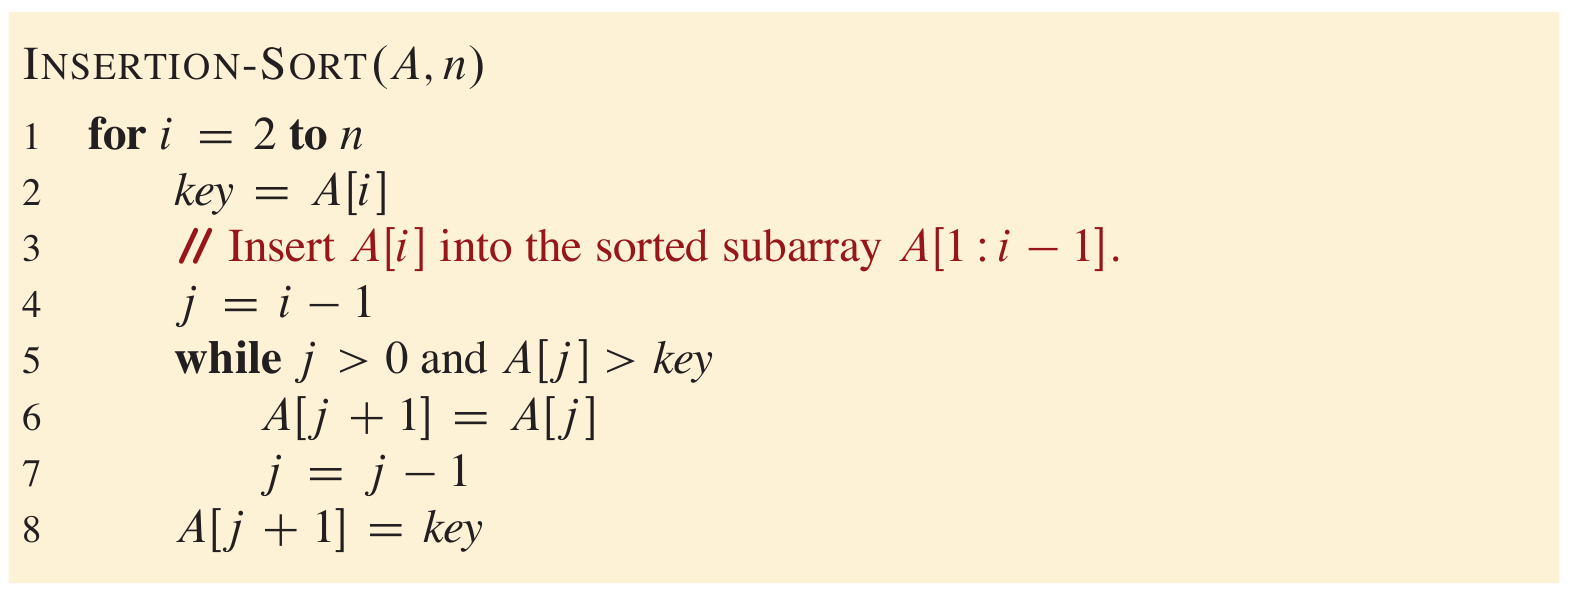
\includegraphics[width=0.7\textwidth]{img/pseudocodigo_insercion.png}
  \caption{Pseudocódigo del ordenamiento por inserción}
  \label{fig:nombre_etiqueta}
\end{figure}  

El ordenamiento por inserción es eficiente para arreglos pequeños o parcialmente ordenados, pero puede volverse ineficiente para arreglos grandes debido a su complejidad cuadrática en el peor de los casos. Sin embargo, es estable y fácil de implementar.

\begin{figure}[h]
  \centering
  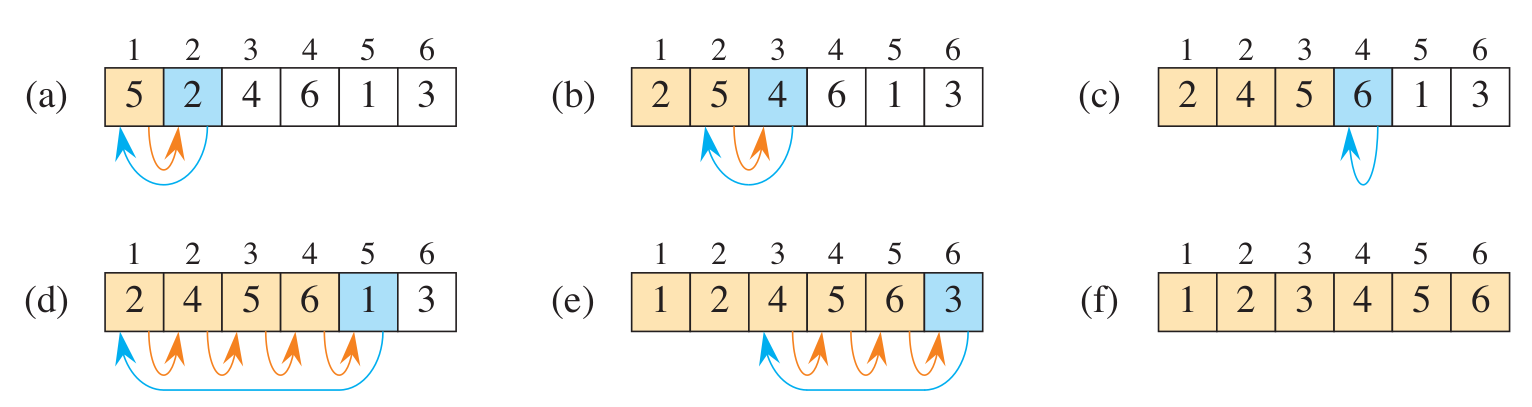
\includegraphics[width=0.8\textwidth]{img/iteraciones_insercion.png}
  \caption{Iteraciones del ordenamiento por inserción}
  \label{fig:nombre_etiqueta}
\end{figure}

Entendido el funcionamiento de este algoritmo, podemos aplicarlo para resolver esta actividad. 
  \begin{itemize}
    \item Comprendamos que nosotros estamos trabajando con un arreglo de objetos, es decir, trabajamos con referencias a objetos que se estan almacenando en cada posición del arreglo.
    \item Las comparaciones se hacen según los atributos de la clase Student, por lo tanto, tenemos la necesidad de usar sus métodos accesores; en este caso solo usamos los métodos getters.
    \item La claridad es mejor que la astucia.
  \end{itemize}

\subsubsection{Commits principales}
%Aqui muestras los commits mas relevantes
%COMMIT----------------------------------------------
  \begin{itemize}
    \item \textbf{Hash: 971ab17de7c8390a9fee07b569b37cbc68cfed6f}
    \item En el presente commit se implementó el algorítmo de ordenamiento de Inserción donde nos aventuramos a diseñar el algoritmo usando nuestra propia lógica. Sim embargo, más adelante encontraremos formas mas eficientes del algoritmo.
  \end{itemize}
    \begin{lstlisting}[language=Java, caption={Commit: Se implementó Quicksort para cui}, numbers=left, firstnumber=1][H]
    public static class InsertionAlgorithmCui (Student[] compañeritos ) {
        int lowest;
        Student pivot;
	for(int i = 0; i < compañeritos.length; i++){
		lowest = i;
		pivot = compañeritos[i];
		while((lowest > 0) && (compañeritos[lowest - 1].getCui() > pivot.getCui())){
			compañeritos[lowest] = compañeritos[lowest - 1];
			lowest--;
		}
		compañeritos[lowest] = pivot;
	    }
     }
    \end{lstlisting}
%COMMIT----------------------------------------------
  \begin{itemize}
    \item \textbf{Hash: 4fe74101fa064fa87663c6f674902add0afde893}
    \item En el presente commit se realizo la elaboración de un metodo privado para comparar Strings haci como se realizo unas modificación al metodo compareEmail() que presento algunos errores anteriormente. 
  \end{itemize}
  \begin{lstlisting}[language=Java, caption={Commit:  Implementando los métodos que usan el algoritmo de inserción para ordenar según nombre y apellidos. Tambien se ha creado un método privado necesario para hacer las comparaciones de los Strings. Por ultimo se corrigió algunos errores de sintaxis y pequeños cambios para mayor comprensión y eficiencia}, numbers=left, firstnumber=1][H]
    
    private static boolean compareString(String word1, String word2){
    	String lower1 = word1.toLowerCase();
    	String lower2 = word1.toLowerCase();
    	int length = lower1.length();
    	if(length > lower2.length()){
    	  length = lower2.length();	
    	}
    	int i = 0;
    	while(i < length){
    	  if(lower1.charAt(i) == lower2.charAt(i)){
		i++;
	      }else{
		if(lower1.charAt(i) > lower2.charAt(i)){
		  return true;
		}
		return false;
	      }
    	}
    	return false;
    }

  \end{lstlisting}

%COMMIT----------------------------------------------
  \begin{itemize}
    \item \textbf{Hash: cda57aa68100e67a2c9f5ac809c67d11b231c28d}
    \item En el presente commit se muestra como se realizo un cambio en el argumento que reciben los metodos , esto debido a el avance realizado en la clase Reader. Se hicieron algunas mejoras en cuanto a la optimización de los metodos. Aunque más adelante encontraremos una forma aún más efectiva para realizar las comparaciones 
  \end{itemize}
  \begin{lstlisting}[language=Java, caption={Commit:   Se cambio el argumento de todos los métodos implementados, de arreglo de Student a arreglo de Reader.Student para posteriormente realizar las pruebas. Por último en colaboracion con las pruebas se corrigieron algunos errores de sintaxis y se eliminó el método convertion porque si el atributo DateOfBirth se compara convirtiendolo a entero, no cumple para todos los casos.}, numbers=left, firstnumber=1][H]
  	
	private static boolean compareString(String word1, String word2){
  	  //Suponemos que los datos no tienen mayusculas donde no deben. Además este método nos
  	  //sirve para ordenar según nacimiento, pues si convertimos a número, no cumple todos los casos
  	 	
		int length = word1.length();
	    	if(length > word2.length()){
	    	  length = word2.length();	
	    	}
	    	int i = 0;
	    	while(i < length){
	    		if(word1.charAt(i) == word2.charAt(i)){
				i++;
			}else{
				if(word1.charAt(i) > word2.charAt(i)){
				  return true;
				}
			return false;
		       }
		}
		return false;
	}
  
  \end{lstlisting}

%COMMIT----------------------------------------------
  \begin{itemize}
    \item \textbf{Hash: 99989865149d77dedee1467670ea5a45529154c4}
    \item En el presente commit encontramos un método mas corto y efectivo de realizar las comparaciones entre strings.Tambien se corrigieron los metodos de Gender y Status a los nuevos parámetros asignados del documento csv. Este metodo se puede implementar para varios parametros, cosa que notaremos más adelante
  \end{itemize}
  \begin{lstlisting}[language=Java, caption={Commit: Algunas correcciones}, numbers=left, firstnumber=1][H]
    
	private static boolean compareString(String word1, String word2){
   		 word1 = word1.toUpperCase();
   		 word2 = word2.toUpperCase();
   		 if (word1.compareTo(word2) <= 0) return false;
   		 return true;
  	}
  \end{lstlisting}


